\subsubsection{UC 2 - Operazioni disponibili nella \texttt{Homepage Agenti}}
\begin{figure}[H]
    \vspace{2em}
    \centering
    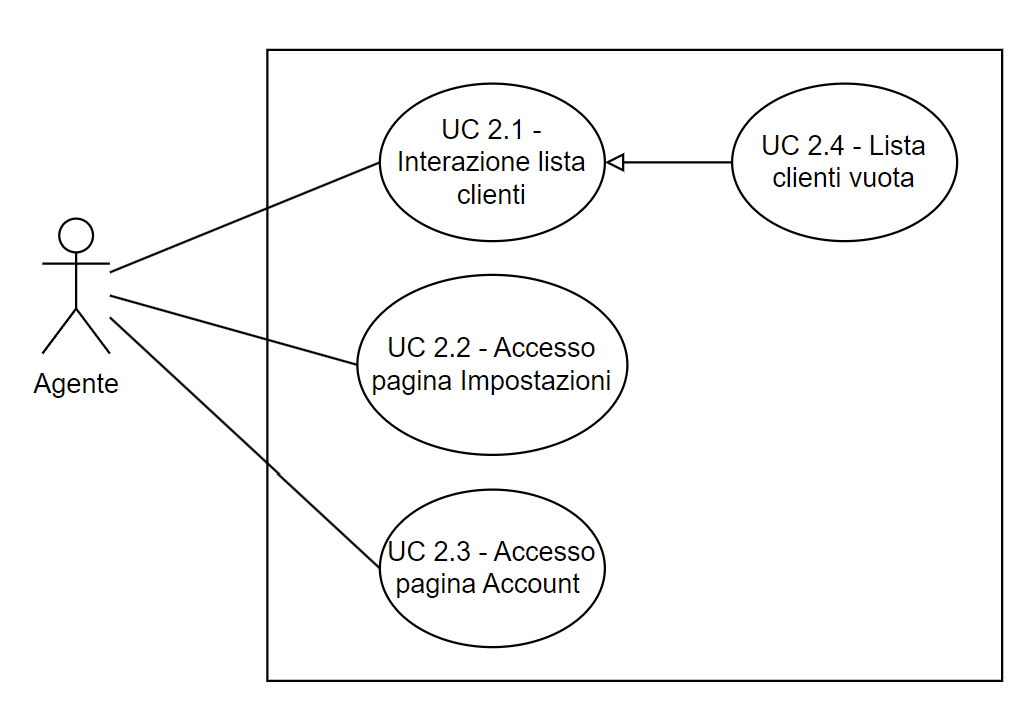
\includegraphics[width=0.75\columnwidth]{img/usecase/UC 2.png}
    \caption{\textit{Use Case} 2: Operazioni disponibili nella \texttt{Homepage Agenti}}
    \label{fig:uc_2}
\end{figure}

\begin{usecase}{ 2.2}{Accesso pagina \texttt{Impostazioni}}
    \usecaseactors{Agente.}
    \usecasedesc{L'agente, cliccando nell'apposito menu il pulsante "Impostazioni", viene spostato nella pagina \texttt{Impostazioni}.}
    \usecasepre{L'utente si è autenticato con successo ed e stato riconosciuto come agente, quindi visualizza la 
                \texttt{Homepage Agenti}.}
    \usecasepost{L'agenti viene spostato nella nella pagina \texttt{Impostazioni}.}
    \usecasescen{
        \begin{itemize}
            \item L'agente visualizza la \texttt{Homepage Agenti};
            \item L'agente visualizza il menu;
            \item L'agente clicca il pulsante "Impostazioni";
            \item L'agente viene spostato nella pagina \texttt{Impostazioni}.
        \end{itemize}}
    \label{uc:uc_2.2}
\end{usecase}

\begin{usecase}{ 2.3}{Accesso pagina \texttt{Account}}
    \usecaseactors{Agente.}
    \usecasedesc{L'agente, cliccando nell'apposito menu il pulsante "\textit{Account}", viene spostato nella pagina \texttt{Account}.}
    \usecasepre{L'utente si è autenticato con successo ed e stato riconosciuto come agente, quindi visualizza la 
                \texttt{Homepage Agenti}.}
    \usecasepost{L'agenti viene spostato nella nella pagina \texttt{Account}.}
    \usecasescen{
        \begin{itemize}
            \item L'agente visualizza la \texttt{Homepage Agenti};
            \item L'agente visualizza il menu;
            \item L'agente clicca il pulsante "\textit{Account}";
            \item L'agente si sposta nella pagina \texttt{Account}.
        \end{itemize}}
    \label{uc:uc_2.3}
\end{usecase}

\begin{usecase}{ 2.4}{Lista clienti vuota}
    \usecaseactors{Agente.}
    \usecasedesc{L'agente che ha una lista clienti vuota visualizza il messaggio 
                 "nessun cliente trovato".}
    \usecasepre{
        \begin{itemize}
            \item L'utente si è autenticato con successo ed e stato riconosciuto come agente, quindi visualizza la 
                \texttt{Homepage Agenti}
            \item La lista clienti è vuota.
        \end{itemize}}
    \usecasepost{L'agente visualizza il messaggio "nessun cliente trovato".}
    \usecasescen{
        \begin{itemize}
            \item L'agente visualizza la \texttt{Homepage Agenti}
            \item La lista clienti è vuota;
            \item L'agente visualizza il messaggio "nessun cliente trovato" al posto della lista.
        \end{itemize}}
    \label{uc:uc_2.4}
\end{usecase}